\begin{center}
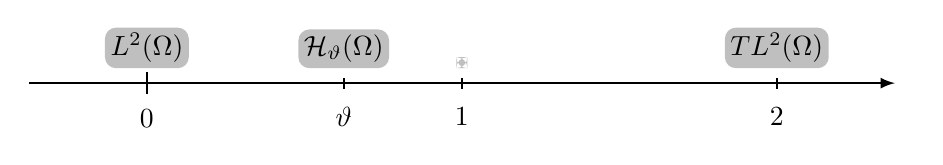
\begin{tikzpicture}[>=latex, thick]
\draw[->] (0,0) -- (11cm,0) node [right] {$\R$};

\draw (1.5,-4pt) -- (1.5,4pt) node[below=10pt]{0};
\draw (1.5,5pt) node[above, align=center, fill=lightgray, rounded corners, inner sep=2pt]{$L^2(\Omega)$};

\draw (4,-2pt) -- (4,2pt);
\draw (4, 5pt) node[above, align=center, fill=lightgray, rounded corners, inner sep=2pt]{$\mathcal{H}_\vartheta(\Omega)$} node[below=10pt]{$\vartheta$};

\draw (5.5,-2pt) -- (5.5,2pt);
\draw (5.5, 5pt) node[above, align=center, fill=lightgray, rounded corners, inner sep=2pt]{$\ns$} node[below=10pt]{1};
\draw (9.5,-2pt) -- (9.5,2pt);
\draw (9.5, 5pt) node[above, align=center, fill=lightgray, rounded corners, inner sep=2pt]{$TL^2(\Omega)$} node[below=10pt]{2};
\end{tikzpicture}
\end{center}